\documentclass{article}

\usepackage{amsmath, graphicx}

\title{Homework3 Report}
\author{Qi Liu}
\date{\today}

\begin{document}
	
\maketitle

\section{Hard Margin SVM}

\subsection{Perpendicular}
The boundary is a hyperplane $w^Tx+b=0$. For any two points $x_1, x_2$ in this hyperplane, we have $w^Tx_1+b=0$ and $w^Tx_2+b=0$. This implies $w^T(x_2-x_1)=0$ which means $w$ is perpendicular to the vector $\overrightarrow{x_1x_2}$. Due to $x_1$ and $x_2$ can be chosen arbitrarily, $w$ is perpendicular to any vector in the hyperplane. Thus $w$ is perpendicular to the hyperplane which is the boundary.

\subsection{Support Vectors}
Due to $x$ is the support vector of the positive class and $y$ is the support vector of the negative class, we have
\begin{align*}
(w^Tx+b)+(w^Ty+b)&=0 \\ w^T(x+y)&=-2b \\ b&=-w^T(x+y)/2
\end{align*}

\subsection{Linear Boundary}
\begin{center}
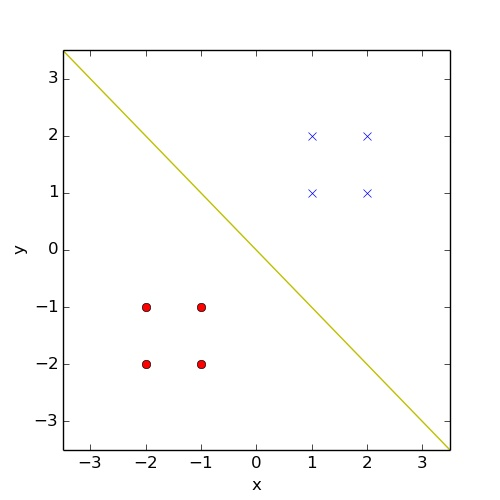
\includegraphics[width=0.5\textwidth]{../result/linear_boundary.jpg}
\end{center}
The boundary is shown as the yellow line in the above figure. The two support vectors are $(-1,-1)$ and $(1, 1)$.

\subsection{Circular Boundary}
\begin{center}
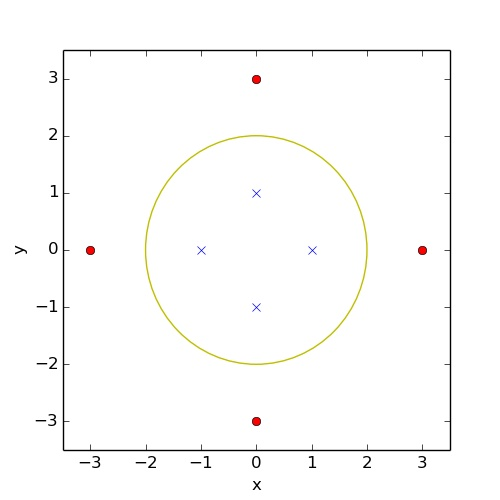
\includegraphics[width=0.5\textwidth]{../result/circular_boundary.jpg}
\end{center}
The boundary is shown as the yellow circle in the above figure. We use the transform $\phi(x)=||x||$ thus kernel is $K(x,x')=||x||\cdot||x'||$. For all positive samples, $\phi(x)=3$. For all negative samples, $\phi(x)=1$. Therefore the boundary is $\phi(x)=2$ which is just the yellow circle.

\section{Soft Margin SVM}

\subsection{Slack Constraint}
Suppose we have a solution with some $\xi_i<0$. If we set $\xi_i=0$, the constraint $$y^{(i)}(w^Tx^{(i)}+b)\ge1-\xi_i$$ will still be satisfied. And the function we want to minimize $$\frac{1}{2}||w||^2+\frac{C}{2}\sum_{i=1}^m\xi_i^2$$ will become smaller. Thus the parameters with $\xi_i<0$ cannot be the optimal solution.

\subsection{Lagrangian}
We can change the original problem to the Lagrangian style. The object function is $$\min_{w,b,\xi}f(w,b,\xi)= \frac{1}{2}||w||^2+\frac{C}{2}\sum_{i=1}^m\xi_i^2$$ and the constraint is $$g_i(w,b,\xi)=-(y^{(i)}(w^Tx^{(i)}+b)-(1-\xi_i)) \le0\quad i=1,\ldots,m.$$ Then the Lagrangian is
\begin{align*}
\mathcal{L}(w,b,\xi,\alpha)&=f(w,b,\xi)+ \sum_{i=1}^m\alpha_ig_i(w,b,\xi) \\
&=\frac{1}{2}w^Tw+\frac{C}{2}\sum_{i=1}^m\xi_i^2 -\sum_{i=1}^m\alpha_i[y^{(i)}(w^Tx^{(i)}+b)-(1-\xi_i)]
\end{align*}
where $\alpha_i\ge0$.

\subsection{Gradients}
By setting the gradient respect to $w$ equal 0 we get
\begin{align*}
\nabla_w\mathcal{L}&=0 \\
\nabla_w\frac{1}{2}w^Tw-\sum_{i=1}^m \nabla_w\alpha_iy^{(i)}w^Tx^{(i)}&=0 \\
w-\sum_{i=1}^m\alpha_iy^{(i)}x^{(i)}&=0 \\
w&=\sum_{i=1}^m\alpha_iy^{(i)}x^{(i)}.
\end{align*}
Calculate the partial derivative respect to $b$,
\begin{align*}
\frac{\partial}{\partial b}\mathcal{L}&=0 \\
-\frac{\partial}{\partial b}\sum_{i=1}^m\alpha_iy^{(i)}b&=0 \\
\sum_{i=1}^m\alpha_iy^{(i)}&=0.
\end{align*}
Take the gradient respect to $\xi$ we get,
\begin{align*}
\nabla_\xi\mathcal{L}&=0 \\
\nabla_w\frac{C}{2}\sum_{i=1}^m\xi_i^2-\sum_{i=1}^m \nabla_w\alpha_i\xi_i&=0 \\
C\xi-\alpha&=0 \\
C\xi&=\alpha \\
\xi&=\frac{\alpha}{C}
\end{align*}
where $\alpha=[\alpha_1,\ldots,\alpha_m]^T$. This implies $\forall i, \xi_i=\frac{\alpha_i}{C}$.

\subsection{Dual Problem}
The objective function is
\begin{align*}
\mathcal{L}(w,b,\xi,\alpha) &=\frac{1}{2}w^Tw+\frac{C}{2}\sum_{i=1}^m\xi_i^2 -\sum_{i=1}^m\alpha_i[y^{(i)}(w^Tx^{(i)}+b)-(1-\xi_i)] \\
&=\frac{1}{2}\sum_{i=1}^m\sum_{j=1}^m(\alpha_iy^{(i)}x^{(i)})^T \alpha_jy^{(j)}x^{(j)}+ \frac{C}{2}\sum_{i=1}^m(\frac{\alpha_i}{C})^2 \\ &\quad-\sum_{i=1}^m\alpha_i[y^{(i)}((\sum_{j=1}^n\alpha_jy^{(j)}x^{(j)})^Tx^{(i)}+b)-(1-\frac{\alpha_i}{C})] \\
&=\frac{1}{2}\sum_{i=1}^m\sum_{j=1}^m\alpha_i\alpha_jy^{(i)} y^{(j)}(x^{(i)})^Tx^{(j)}+\frac{1}{2C}\sum_{i=1}^m\alpha_i^2 \\
&\quad-\sum_{i=1}^m\sum_{j=1}^m\alpha_i\alpha_jy^{(i)} y^{(j)}(x^{(i)})^T x^{(j)}-\sum_{i=1}^m(\alpha_iy^{(i)}b-\alpha_i+\frac{a_i^2}{C}) \\
&=\sum_{i=1}^m\alpha_i-\frac{1}{2}\sum_{i=1}^m\sum_{j=1}^m\alpha_i \alpha_jy^{(i)}y^{(j)}(x^{(i)})^Tx^{(j)}- \frac{1}{2C}\sum_{i=1}^m\alpha_i^2
\end{align*}
Therefore the dual problem is $$\max_\alpha \sum_{i=1}^m\alpha_i-\frac{1}{2}\sum_{i=1}^m\sum_{j=1}^m\alpha_i \alpha_jy^{(i)}y^{(j)}(x^{(i)})^Tx^{(j)}- \frac{1}{2C}\sum_{i=1}^m\alpha_i^2$$ with the constraints $$\forall i,\alpha_i\ge0$$ and $$\sum_{i=1}^m\alpha_iy^{(i)}=0.$$

\section{Spam Email Filter}
We use a Python library based on LibSVM to do the spam email filter. Three kernel functions are used and all the results are shown below. We did not show all the parameters because there are too many.
\begin{center}
\begin{tabular}{|c|c|c|c|}
\hline \bf{Kernel} & linear & polynomial & rbf \\
\hline \bf{Accuracy} & 89.3\% & 80.3\% & 90.8\% \\
\hline \bf{Precision} & 87.5\% & 90.7\% & 88.3\% \\
\hline \bf{Recall} & 84.4\% & 54.7\% & 87.9\% \\
\hline
\end{tabular}
\end{center}

\end{document}